\documentclass[12pt,letterpaper,twocolumn,openany,nodeprecatedcode,bg=none]{dndbook}
\usepackage[english]{babel}
\usepackage[utf8]{inputenc}
\usepackage{longtable,booktabs,array}
\usepackage{calc}
\usepackage{etoolbox}
\usepackage{caption}
\AtBeginEnvironment{longtable}{\small}

% Fix for Pandoc 3.1.7+ image handling
\providecommand{\pandocbounded}[1]{#1}

% Pandoc's compact list helper
\providecommand{\tightlist}{%
  \setlength{\itemsep}{0pt}\setlength{\parskip}{0pt}}

% Remove "Figure N:" prefix from captions
\captionsetup{labelformat=empty}

% Remove section numbering
\setcounter{secnumdepth}{0}

\begin{document}

\title{Psionic}
\author{Class Handbook}
\date{}
\maketitle

\onecolumn

\emph{Your trusty class handbook for the Old Scrolls roleplaying game.}

\clearpage

\begin{figure}
\centering
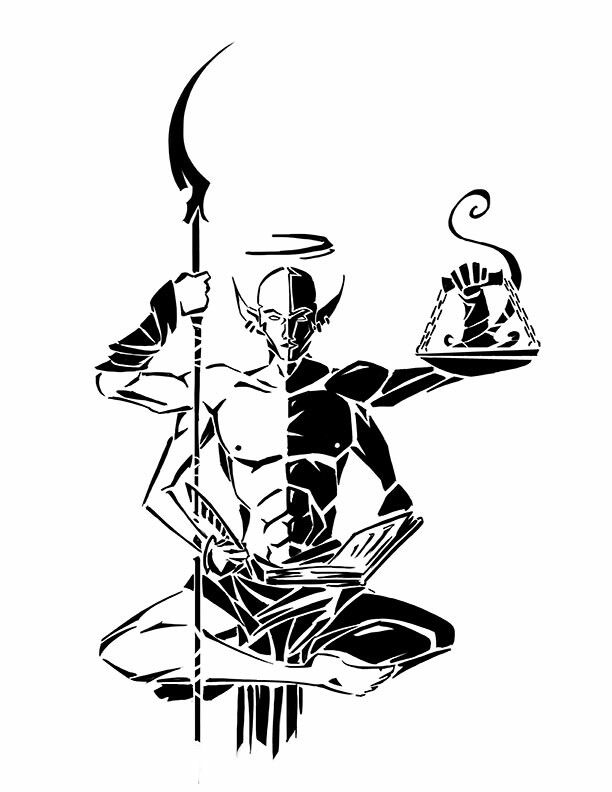
\includegraphics[width=1\linewidth,height=\textheight,keepaspectratio]{vivec.jpg}
\caption{\emph{A psionic has mastery over mind and matter}}
\end{figure}

\clearpage

\section{Psionic}\label{psionic}

The psionic harnesses magical powers poorly understood that draw upon
the sheer willpower of the mortal soul and mind. They specialize in
telekinesis, but also are known to be able to use their mastery over
minds and souls to perform even stranger feats of magic.

\subsection{Core Psionic Traits}\label{core-psionic-traits}

\begin{longtable}[]{@{}
  >{\raggedright\arraybackslash}p{(\linewidth - 2\tabcolsep) * \real{0.2542}}
  >{\raggedright\arraybackslash}p{(\linewidth - 2\tabcolsep) * \real{0.7458}}@{}}
\toprule\noalign{}
\begin{minipage}[b]{\linewidth}\raggedright
\textbf{Primary Ability}
\end{minipage} & \begin{minipage}[b]{\linewidth}\raggedright
Wisdom
\end{minipage} \\
\midrule\noalign{}
\endhead
\bottomrule\noalign{}
\endlastfoot
\textbf{Hit Points} & 12 at 1st level, 8 per level gained after 1st \\
\textbf{Saving Throw Proficiencies} & Dexterity, Wisdom \\
\textbf{Skill Proficiencies} & Choose any 2 skills. If you choose a
skill you already have, you gain expertise with it. \\
\textbf{Weapon Proficiencies} & Choose 1: Blade, Blunt, Bow, Mechanical,
Polearm, and Shield \\
\textbf{Starting Equipment} & Tunic, Staff, Dagger \\
\end{longtable}

\subsection{Psionic Features Table}\label{psionic-features-table}

\begin{longtable}[]{@{}
  >{\raggedright\arraybackslash}p{(\linewidth - 6\tabcolsep) * \real{0.0704}}
  >{\raggedright\arraybackslash}p{(\linewidth - 6\tabcolsep) * \real{0.1549}}
  >{\raggedright\arraybackslash}p{(\linewidth - 6\tabcolsep) * \real{0.0423}}
  >{\raggedright\arraybackslash}p{(\linewidth - 6\tabcolsep) * \real{0.7324}}@{}}
\toprule\noalign{}
\begin{minipage}[b]{\linewidth}\raggedright
Level
\end{minipage} & \begin{minipage}[b]{\linewidth}\raggedright
Proficiency
\end{minipage} & \begin{minipage}[b]{\linewidth}\raggedright
Psi
\end{minipage} & \begin{minipage}[b]{\linewidth}\raggedright
Class Features
\end{minipage} \\
\midrule\noalign{}
\endhead
\bottomrule\noalign{}
\endlastfoot
1 & +2 & 2 & Psionic Defense, Psionic Power, Psionic Strike (1d6) \\
2 & +2 & 2 & Psionic Discipline \\
3 & +2 & 3 & Psionic Strike (1d8) \\
4 & +2 & 3 & Ability Score Improvement, Psionic Discipline \\
5 & +3 & 4 & Psionic Strike (1d10) \\
6 & +3 & 4 & Psionic Discipline \\
7 & +3 & 4 & Psionic Strike (1d12) \\
8 & +3 & 4 & Ability Score Improvement, Psionic Discipline \\
9 & +4 & 5 & Invigorating Flow \\
10 & +4 & 5 & Master of Psionics \\
\end{longtable}

\twocolumn

\subsection{Psionic Features}\label{psionic-features}

As a psionic, you gain the following class features when you reach the
specified levels. These features are listed on the Psionic Features
table.

\subsection{Level 1: Psionic Defense}\label{level-1-psionic-defense}

While you aren't wearing armor, your AC is 10 + your Dexterity modifier
+ your Wisdom modifier.

\subsection{Level 1: Psionic Power}\label{level-1-psionic-power}

You have learned to tap into psionic energy, a life force that allows
you to complete incredible feats of power.

On your turn as a magic action, you can focus your psionic energy. You
gain psi points based on your level as detailed on the Psionic Features
table. You can spend those points to activate disciplines. You retain
psi points until you spend them or until the start of your next turn.

Some disciplines specify that you take an action when you spend them.
These actions are in addition to your normal action and move. Other
disciplines specify that you use them on another creature's turn. As
long as you have the psi points needed to use the discipline, you can
use it.

Other disciplines require a saving throw. The save DC is 8 + your
proficiency bonus + your Wisdom modifier.

You gain the Swift Strike psionic discipline and one other discipline of
your choice.

\subsection{Level 1: Psionic Strike}\label{level-1-psionic-strike}

Your unarmed strikes inflict 1d6 force damage. When you make an unarmed
strike, you can choose to use your Wisdom modifier in place of Strength
to modify your attack and damage rolls.

If you are proficient with a weapon, you can attack with it when you
would make an unarmed strike. However, you must replace its damage die
with the die granted to your unarmed strike by this feature.

\subsection{Level 2: Psionic
Discipline}\label{level-2-psionic-discipline}

You gain an additional psionic discipline. Each time you gain a level,
you can swap one discipline you know for another one.

\subsection{Level 3: Psionic Strike}\label{level-3-psionic-strike}

Your unarmed strikes now inflict 1d8 force damage. Pick one of the
following damage types: fire, lightning, or thunder. You can choose to
inflict force or the chosen damage type each time you hit a target with
an unarmed strike.

\subsection{Level 4: Ability Score
Improvement}\label{level-4-ability-score-improvement}

You gain a +1 bonus to two abilities of your choice.

\subsection{Level 4: Psionic
Discipline}\label{level-4-psionic-discipline}

You gain an additional psionic discipline. Each time you gain a level,
you can swap one discipline you know for another one.

\subsection{Level 5: Psionic Strike}\label{level-5-psionic-strike}

Your unarmed strikes now inflict 1d10 force damage. If you miss with an
unarmed strike, the target still takes damage of your strike's type
equal to your Wisdom modifier.

\subsection{Level 6: Psionic
Discipline}\label{level-6-psionic-discipline}

You gain an additional psionic discipline. Each time you gain a level,
you can swap one discipline you know for another one.

\subsection{Level 7: Psionic Strike}\label{level-7-psionic-strike}

Your unarmed strikes now inflict 1d12 force damage. When rolling damage
for your unarmed strike against an object, treat any dice you roll as if
they rolled the maximum damage possible.

\subsection{Level 8: Ability Score
Improvement}\label{level-8-ability-score-improvement}

You gain a +1 bonus to two abilities of your choice.

\subsection{Level 8: Psionic
Discipline}\label{level-8-psionic-discipline}

You gain an additional psionic discipline. Each time you gain a level,
you can swap one discipline you know for another one.

\subsection{Level 9: Invigorating Flow}\label{level-9-invigorating-flow}

When you focus your psionic energy while you are at half hit points or
less, you regain hit points equal to 1d8 + the psi you gained.

\subsection{Level 10: Master of
Psionics}\label{level-10-master-of-psionics}

When you focus your psionic energy, you can choose to gain double the
psi you normally gain. Once you use this feature, you cannot use it
again until you finish a long rest.

\section{Psionic Disciplines}\label{psionic-disciplines}

Here are psionic disciplines you can choose from.

\subsection{Astral Walk}\label{astral-walk}

\textbf{Psionic Discipline}

Spend 2 psi on your turn. You can fly until the end of the turn. You
fall if you end the turn in midair.

\subsection{Inevitable Strike}\label{inevitable-strike}

\textbf{Psionic Discipline}

Spend 1 psi on any turn. The next attack you make this turn hits. Roll
the attack to see if it is a critical hit.

\subsection{Kinetic Push}\label{kinetic-push}

\textbf{Psionic Discipline}

When you hit a target with a melee attack, spend 1 or more psi to push
the target up to 10 feet once per psi spent.

\subsection{Kinetic Slam}\label{kinetic-slam}

\textbf{Psionic Discipline}

When you hit a target with a melee attack, spend 1 psi to knock the
target prone. If the target is larger than you, it also takes force
damage equal to your level.

\subsection{Mental Fortress}\label{mental-fortress}

\textbf{Psionic Discipline}

Spend 1 psi on your turn to gain +2 AC until your next turn. If you
already benefit from this discipline's AC bonus, the bonus is instead
+1.

\subsection{Mind Shatter}\label{mind-shatter}

\textbf{Psionic Discipline}

When you hit a target with a melee attack, spend 1 or more psi. For each
psi spent, the target takes psychic damage equal to a roll of your
unarmed strike damage die + your Wisdom modifier.

\subsection{Mind Stun}\label{mind-stun}

\textbf{Psionic Discipline}

Spend 4 psi and make an unarmed strike on your turn. If you hit, the
target must make a Constitution save. If it fails, it cannot use actions
on its next turn. If it succeeds, it automatically succeeds on saves
against this discipline for the next hour.

\subsection{Phase Shift}\label{phase-shift}

\textbf{Psionic Discipline}

Spend 1 psi on your turn or at the start of another creature's turn. You
move once.

\subsection{Reactive Ward}\label{reactive-ward}

\textbf{Psionic Discipline}

When you take damage from an attack, spend 1 psi and roll 1d10 + your
Wisdom modifier + your psionic level. Reduce the damage by that amount.
If you reduce the damage to 0, you may pick a creature in melee range
including the attacker. It takes the original damage.

\subsection{Silent Mind}\label{silent-mind}

\textbf{Psionic Discipline}

Spend 1 psi on your turn. Until your next turn, you are completely
silent. While silent in this manner you are hidden, no check necessary,
from creatures that cannot see you. You can still make noise if you wish
to, but doing so ends this effect.

\subsection{Swift Strike}\label{swift-strike}

\textbf{Psionic Discipline}

Spend 1 psi on your turn to make an unarmed strike as an attack action.

\subsection{Vital Surge}\label{vital-surge}

\textbf{Psionic Discipline}

While you are at half hit points or less on your turn, spend 1 psi to
regain 1d6 + your Wisdom modifier hit points.

\subsection{Weightless Step}\label{weightless-step}

\textbf{Psionic Discipline}

Spend 1 psi on any turn. When you move this turn, you may move across
liquids and along vertical surfaces as part of this move and ignore
difficult terrain. You sink or fall at the end of your turn.

\onecolumn

\begin{figure}
\centering
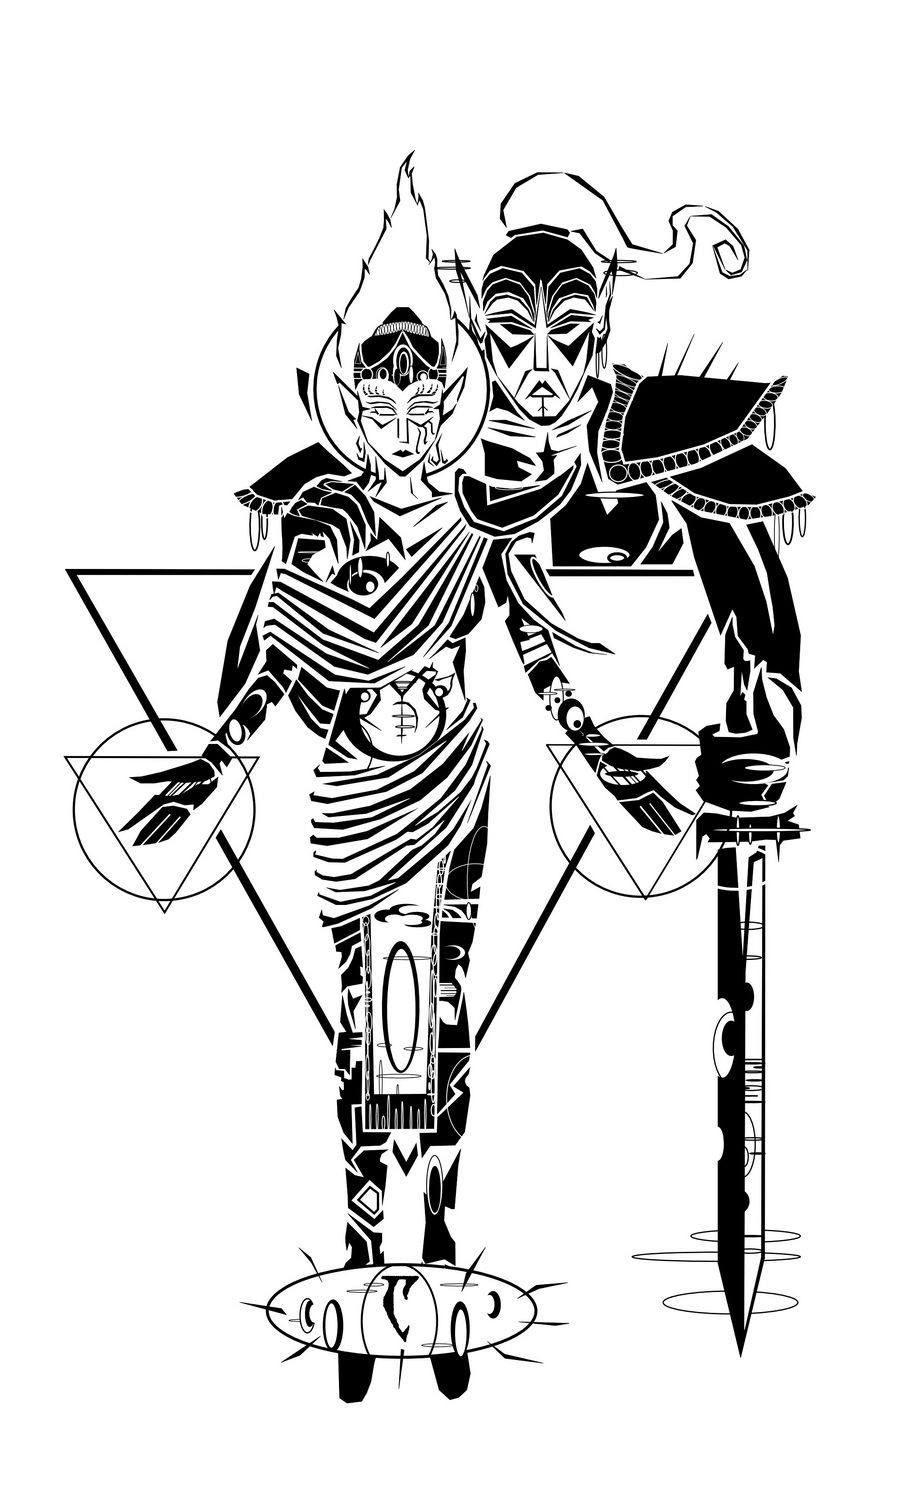
\includegraphics[width=1\linewidth,height=\textheight,keepaspectratio]{almalexia.jpg}
\caption{\emph{A psionic unbound is a threat like no other}}
\end{figure}

\end{document}